\subsection{Depth Map Estimation}
A blender script was created to generate randomized 3D situations for analysis. This stochastic approach generates a large number of 3D scene environments and their associated depth maps.
Through this training, we aim to obtain a neural network that takes input as stereo images and output the depth parity. This depth parity would later used as part of the short-term path planner in the control policy.
Shapenet \cite{shapenet2015}, an annotated, large-scale dataset of 3D shapes was used as obstacles in the training phase of the CNN for depth parity estimation, and as the obstacles for the agent to circumnavigate in the test phase.

\begin{figure}
  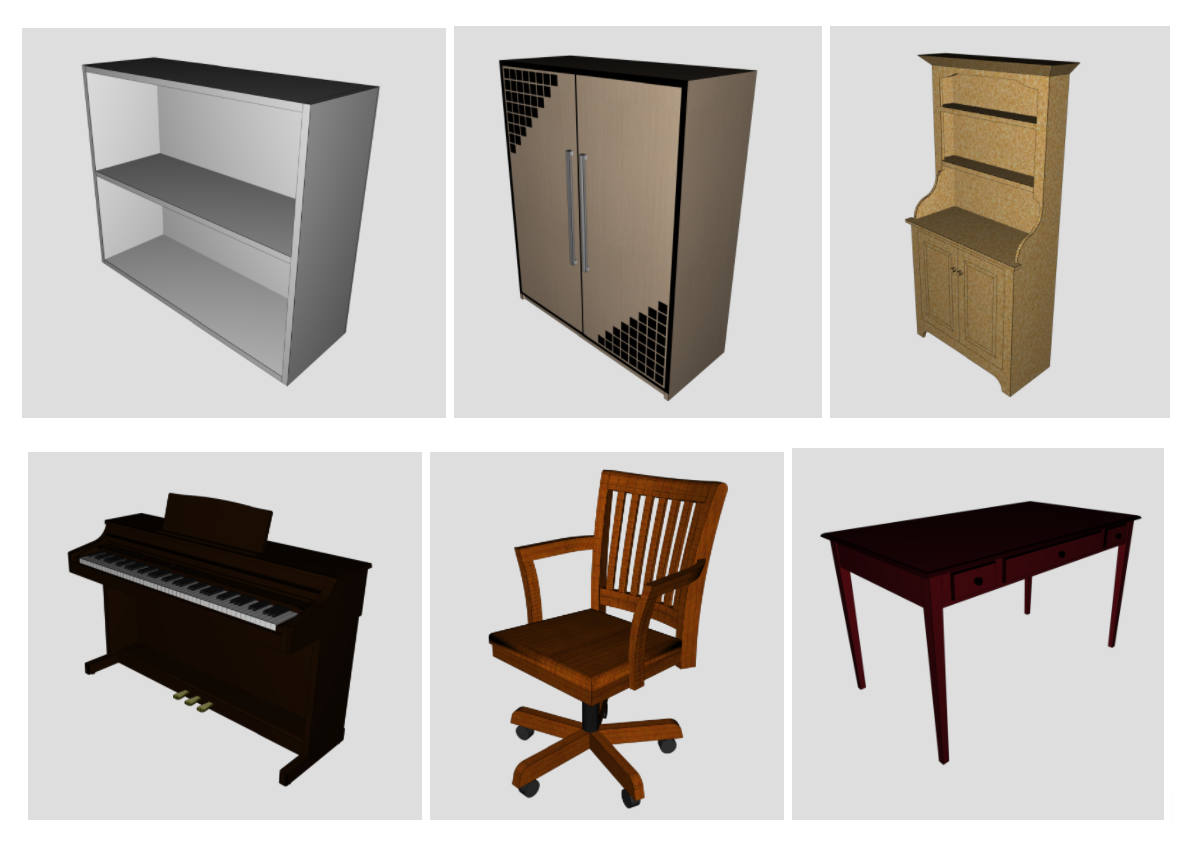
\includegraphics[width=\linewidth]{images/shapenet.png}
  \caption{Shapenet Dataset}
  \label{fig:boat1}
\end{figure}

A dataset of 20,000 training examples was generated using 3D models from the Shapenet dataset. For each example, 8-10 models were chosen at random and placed in the scene.
The placement and rotation of each model is random, and 3 scenes are rendered:

\begin{figure}[!htb]
  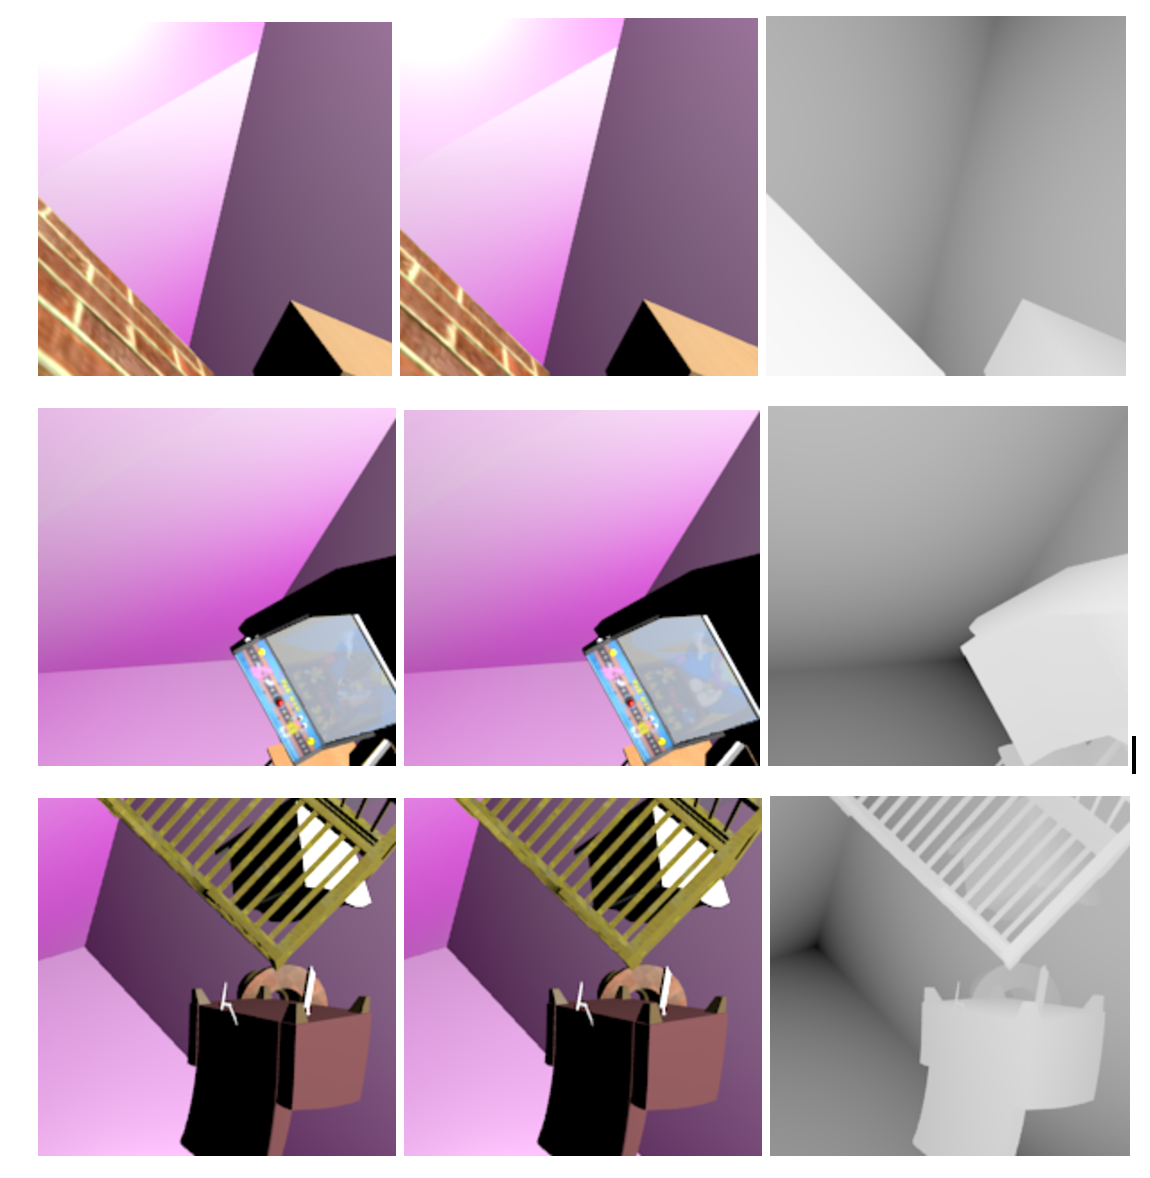
\includegraphics[width=\linewidth]{images/depthmap1.png}
  \caption{Depth map estimation}
  \label{fig:boat1}
\end{figure}

\begin{enumerate}
\item Left camera stereo image
\item Right camera stereo image
\item Depth map
\end{enumerate}
This dataset of 20,000 images was normalized along each pixel to aid the training process.

A Convolutional Neural Network for estimating depth maps using a stereo image pair was trained. The network accepts as input 2 grayscale images and produces an estimate of the depth map corresponding to the images \cite{MayerIHFCDB15} \cite{foucard_2016}.
A loss function of mean squared error was used to as the objective. The network was trained using an Adam Optimizer \cite{KingmaB14}, with learning rate 0.01. Hold out validation with split 10\%  was performed i.e 18,000 training examples were used as the training set and 2000 as validation set. The validation loss and training loss at each epoch were recorded. The training was halted once validation loss did not improve significantly.
Loss function used:
\[ L(x_n,y_n) = {\sum_{i=1}^{200}\sum_{j=1}^{200}} (y_{ij} - x_{ij})^2 \]